% !TeX root = main.tex
\chapter{Experiments and Results}
\label{ch:results}

This chapter presents the quantitative results in the order of the \glspl{rq}. Sections~\ref{sec:results-models} and~\ref{sec:results-reconstruction} answer \gls{rq}~1 with the encoders, initializations, and line reconstructions of the pipelines on U-DIADS-TL and DIVA-HisDB. Section~\ref{sec:results-rq2} reduces the number of training pages for \gls{rq}~2, and Section~\ref{sec:results-rq3} evaluates the transfer to other collections for \gls{rq}~3. All metrics are given in percent, and higher values are better.

% Keep the table spacing compact without stretching it to fill each page.
\begingroup
\raggedbottom
\setlength{\intextsep}{6pt}
\setlength{\floatsep}{6pt}
\setlength{\textfloatsep}{8pt}
\setlength{\LTpre}{6pt}
\setlength{\LTpost}{6pt}

\FloatBarrier

\section{Encoders and Initializations}
\label{sec:results-models}

The models of this section are trained on the complete benchmark partitions. On both benchmarks, the best pipelines reach or exceed the published \gls{sota}. Additionally, the initialization has a larger effect than the choice of the encoder.

\subsection{Benchmark Results}
\label{sec:results-rq11}

As shown in Table~\ref{tab:rq1-mean}, the best configurations outperform the published results on both benchmarks. On U-DIADS-TL, Mask R-CNN with CATMuS-initialized ConvNeXt-Tiny reaches 92.03\%, compared with 83.00\% for PERO, the best result of the FEST competition~\cite{Zottin_2025_FEST}. The U-Net with projection cuts also exceeds PERO with 87.38\%. On DIVA-HisDB, Mask R-CNN reaches 99.21\%, and seven of its seventeen configurations exceed the 97.43\% of Mask R-CNN+~\cite{signals3030032}. The results per subset and for all five metrics are given in Appendix~\ref{app:rq1-subsets}.

\begin{table}[htbp]
    \centering
    \footnotesize
    \setlength{\tabcolsep}{3.5pt}
    \caption{Mean line \gls{fm} of the three pipelines for every encoder and initialization.}
    \label{tab:rq1-mean}
    \begin{tabular}{@{}llcccccc@{}}
        \toprule
        & & \multicolumn{3}{c}{U-DIADS-TL} & \multicolumn{3}{c}{DIVA-HisDB} \\
        \cmidrule(lr){3-5}\cmidrule(l){6-8}
        Encoder & Initialization & U-Net & RT-DETR & \shortstack{Mask\\R-CNN} & U-Net & RT-DETR & \shortstack{Mask\\R-CNN} \\
        \midrule
        ConvNeXt-Tiny & Random             & 79.89 & 33.39 & 78.00 & 91.64 & 89.76 & 94.51 \\
                      & ImageNet           & \textbf{87.38} & 83.86 & 91.87 & 95.03 & 91.18 & 98.43 \\
                      & DINOv3 (LVD-1689M) & 85.81 & 42.23 & 91.64 & \textbf{95.76} & 85.15 & \textbf{99.21} \\
                      & DINOv3 (cBAD)      & --    & 69.10 & 90.22 & --    & 88.98 & 98.87 \\
                      & CATMuS             & --    & 90.44 & \textbf{92.03} & --    & 93.34 & 98.58 \\
        \midrule
        PVTv2-B2      & Random             & 79.16 & 62.15 & 88.25 & 89.07 & 88.47 & 96.97 \\
                      & ImageNet           & 87.00 & 80.55 & 91.37 & 91.82 & 91.22 & 98.95 \\
                      & DINOv3 (cBAD)      & --    & 69.29 & 91.01 & --    & 91.83 & 98.54 \\
                      & CATMuS             & --    & \textbf{90.80} & 91.77 & --    & 91.86 & 99.14 \\
        \midrule
        ViT-Small     & Random             & 82.97 & 44.79 & 86.64 & 89.17 & 91.96 & 90.77 \\
                      & ImageNet           & 84.04 & 70.17 & 90.08 & 92.73 & 89.58 & 94.62 \\
                      & DINOv3 (LVD-1689M) & 86.38 & 78.95 & 88.02 & 90.04 & 90.08 & 88.20 \\
                      & DINOv3 (cBAD)      & --    & 73.09 & 89.54 & --    & 89.49 & 95.41 \\
                      & CATMuS             & --    & 90.37 & 91.18 & --    & \textbf{93.40} & 97.43 \\
        \midrule
        \multicolumn{2}{@{}l}{PERO (FEST 2025)~\cite{Zottin_2025_FEST}} & \multicolumn{3}{c}{83.00} & \multicolumn{3}{c}{--} \\
        \multicolumn{2}{@{}l}{VAI-OCR (FEST 2025)~\cite{Zottin_2025_FEST}} & \multicolumn{3}{c}{74.80} & \multicolumn{3}{c}{--} \\
        \multicolumn{2}{@{}l}{Conn.-Aware U-Net++~\cite{sterzinger2025fewshot}} & \multicolumn{3}{c}{61.40} & \multicolumn{3}{c}{--} \\
        \multicolumn{2}{@{}l}{APAU-Net~\cite{Beghoura2026-dp}} & \multicolumn{3}{c}{63.35} & \multicolumn{3}{c}{54.94} \\
        \multicolumn{2}{@{}l}{Mask R-CNN~\cite{signals3030032}} & \multicolumn{3}{c}{--} & \multicolumn{3}{c}{76.60} \\
        \multicolumn{2}{@{}l}{Mask R-CNN+~\cite{signals3030032}} & \multicolumn{3}{c}{--} & \multicolumn{3}{c}{97.43} \\
        \bottomrule
    \end{tabular}
\end{table}

\label{sec:results-rq12}\label{sec:results-rq13}
The effect of the initialization differs between the pipelines. With random initialization, RT-DETR + BBox U-Net reaches only 33.39\% on U-DIADS-TL. With CATMuS initialization, all three of its encoders reach 90.37--90.80\%. Mask R-CNN and the U-Net with projection cuts depend less on the initialization. However, random initialization also gives their lowest U-DIADS-TL results, with 78.00\% and 79.89\% for ConvNeXt-Tiny. For all pipelines, Syr341 is the most difficult subset.

\FloatBarrier

\subsection{Comparison by Factors}
\label{sec:results-rq1-summary}

As shown in Tables~\ref{tab:rq1-grouped} and~\ref{tab:rq1-factor-ranges}, the encoder family has a smaller effect than the initialization. No encoder family is the best in all pipelines, and the family changes the mean line \gls{fm} over both benchmarks by 2.49 to 6.53 percentage points. The initialization changes it by 4.35 to 23.28 points. The largest effect occurs for RT-DETR + BBox U-Net, where CATMuS improves the U-DIADS-TL result by 6.58--20.20 percentage points over ImageNet with the same encoder. The encoder size has a small effect as well. Larger encoders improve the U-DIADS-TL result of the U-Net with projection cuts and Mask R-CNN by only 1.6 and 1.5 percentage points (Appendix~\ref{app:rq1-size}). The standard deviations in Table~\ref{tab:rq1-grouped} show the variation between configurations, not between repeated training runs.

\begin{table}[htbp]
    \centering
    \footnotesize
    \setlength{\tabcolsep}{3pt}
    \caption{Mean line \gls{fm} by initialization and encoder family, pooled over both benchmarks (mean \(\pm\) standard deviation over \(n\) results).}
    \label{tab:rq1-grouped}
    \begin{tabular}{@{}llrcrcrc@{}}
        \toprule
        & & \multicolumn{2}{c}{U-Net} & \multicolumn{2}{c}{RT-DETR} & \multicolumn{2}{c}{Mask R-CNN} \\
        \cmidrule(lr){3-4}\cmidrule(lr){5-6}\cmidrule(l){7-8}
        Factor & Group & \(n\) & \gls{fm} & \(n\) & \gls{fm} & \(n\) & \gls{fm} \\
        \midrule
        Initialization & Random             & 6 & 85.32\,\(\pm\)\,5.33 & 6 & 68.42\,\(\pm\)\,25.44 & 6 & 89.19\,\(\pm\)\,6.69 \\
                       & ImageNet           & 6 & \textbf{89.67}\,\(\pm\)\,4.17 & 6 & 84.43\,\(\pm\)\,8.21 & 6 & 94.22\,\(\pm\)\,3.77 \\
                       & DINOv3 (LVD-1689M) & 4 & 89.50\,\(\pm\)\,4.58 & 4 & 74.10\,\(\pm\)\,21.73 & 4 & 91.77\,\(\pm\)\,5.23 \\
                       & DINOv3 (cBAD)      & -- & -- & 6 & 80.30\,\(\pm\)\,10.88 & 6 & 93.93\,\(\pm\)\,4.23 \\
                       & CATMuS             & -- & -- & 6 & \textbf{91.70}\,\(\pm\)\,1.40 & 6 & \textbf{95.02}\,\(\pm\)\,3.73 \\
        \midrule
        Encoder family & ConvNeXt & 6 & \textbf{89.25}\,\(\pm\)\,6.07 & 10 & 76.74\,\(\pm\)\,21.71 & 10 & 93.34\,\(\pm\)\,6.43 \\
                       & PVTv2    & 4 & 86.76\,\(\pm\)\,5.44 & 8 & \textbf{83.27}\,\(\pm\)\,11.61 & 8 & \textbf{94.50}\,\(\pm\)\,4.35 \\
                       & ViT      & 6 & 87.56\,\(\pm\)\,3.75 & 10 & 81.19\,\(\pm\)\,15.22 & 10 & 91.19\,\(\pm\)\,3.53 \\
        \bottomrule
    \end{tabular}
\end{table}

\begin{table}[htbp]
    \centering
    \caption{Range of the pooled mean \gls{fm} across encoder families and initializations, and best mean \gls{fm}.}
    \label{tab:rq1-factor-ranges}
    \small
    \setlength{\tabcolsep}{4pt}
    \begin{tabular}{@{}lccccc@{}}
        \toprule
        & \multicolumn{2}{c}{Pooled range (percentage points)} & \multicolumn{2}{c}{Best mean \gls{fm}} \\
        \cmidrule(lr){2-3}\cmidrule(l){4-5}
        Pipeline & Encoder family & Initialization & U-DIADS-TL & DIVA-HisDB \\
        \midrule
        \multicolumn{5}{@{}l}{\emph{Semantic segmentation}} \\
        U-Net & 2.49 & 4.35 & 87.38 & 95.76 \\
        \multicolumn{5}{@{}l}{\emph{Instance segmentation}} \\
        RT-DETR + BBox U-Net & 6.53 & 23.28 & 90.80 & 93.40 \\
        Mask R-CNN & 3.31 & 5.83 & \textbf{92.03} & \textbf{99.21} \\
        \bottomrule
    \end{tabular}
\end{table}

\FloatBarrier
\section{Line Reconstruction}
\label{sec:results-reconstruction}

In the detection-based pipelines, the segmentation inside the boxes limits the result more than the detection of the lines.

\label{sec:results-components}
As shown in Table~\ref{tab:rq1-twostage-components}, the RT-DETR detector finds most DIVA-HisDB lines, with a box F1 of 93.24--97.89\% at an \gls{iou} of 0.5. However, \gls{gt} boxes and \gls{gt} masks improve the line \gls{fm} by the same amount, from 93.34\% to 96.03\% and 95.99\%. On DIVA-HisDB, both stages therefore contribute to the remaining error.

\begin{table}[htbp]
    \centering
    \caption{Components of RT-DETR + BBox U-Net on DIVA-HisDB (ConvNeXt-Tiny, CATMuS).}
    \label{tab:rq1-twostage-components}
    \footnotesize
    \setlength{\tabcolsep}{3pt}
    \begin{tabular}{@{}lcccccccc@{}}
        \toprule
        & \multicolumn{3}{c}{Detector boxes} & Crop & \multicolumn{4}{c}{Line-level \gls{fm}} \\
        \cmidrule(lr){2-4}\cmidrule(lr){5-5}\cmidrule(l){6-9}
        Subset & F1@0.5 & F1@0.75 & AP@0.5 & IoU & Pipeline & GT boxes & GT masks & GT export \\
        \midrule
        CB55 & 97.89 & 95.42 & 83.61 & 91.91 & 97.71 & 99.84 & 98.06 & 96.52 \\
        CS18 & 93.24 & 87.75 & 87.00 & 88.73 & 92.54 & 96.23 & 93.72 & 95.00 \\
        CS863 & 96.00 & 92.48 & 86.18 & 85.71 & 89.75 & 92.02 & 96.18 & 96.69 \\
        \midrule
        Mean & 95.71 & 91.88 & 85.59 & 88.78 & 93.34 & 96.03 & 95.99 & 96.07 \\
        \bottomrule
    \end{tabular}
\end{table}

\label{sec:results-integration}\label{app:boundary-reconstruction}\label{sec:results-dp-seam}
The second stage has the largest effect when the \gls{gt} is pixel-accurate (Table~\ref{tab:second-stage}). With identical Mask R-CNN detections, the BBox U-Net raises the U-DIADS-TL \gls{fm} from 16.61\% with the coarse \gls{roi} masks to 90.82\%. On DIVA-HisDB, only the ink inside a polygon is evaluated, and the \gls{roi} masks reach 98.58\%. Here, the \gls{dp} seam raises the result to 99.55\%. However, the seam region has to match the \gls{gt} format. On U-DIADS-TL, its filled region lowers the \gls{fm} to 67.85\%, and only its intersection with the predicted ink reaches 90.66\%, which is close to the 90.82\% of the BBox U-Net.

\begin{table}[htbp]
    \centering
    \scriptsize
    \setlength{\tabcolsep}{3pt}
    \caption{Second stages and \gls{dp} seam for the same Mask R-CNN detections (line \gls{fm}).}
    \label{tab:second-stage}
    \begin{tabular*}{\textwidth}{@{\extracolsep{\fill}}llcccccccc@{}}
        \toprule
        & & \multicolumn{4}{c}{DIVA-HisDB} & \multicolumn{4}{c}{U-DIADS-TL} \\
        \cmidrule(lr){3-6}\cmidrule(l){7-10}
        Second stage & Output & CB55 & CS18 & CS863 & Mean & Lat.\,14396 & Lat.\,2 & Syr.\,341 & Mean \\
        \midrule
        \glsentryshort{roi} mask (28$\times$28) & mask & 98.36 & 97.87 & 99.50 & 98.58 & 33.43 & 12.88 & 3.52 & 16.61 \\
        BBox U-Net & mask & 99.03 & 99.04 & 99.17 & 99.08 & \textbf{95.47} & \textbf{93.14} & 83.84 & \textbf{90.82} \\
        \midrule
        \multicolumn{10}{@{}l}{\emph{Postprocessing of the BBox U-Net output}} \\
        + \gls{dp} seam & region & \textbf{99.20} & \textbf{99.44} & \textbf{100.00} & \textbf{99.55} & 90.18 & 78.61 & 34.77 & 67.85 \\
        + \gls{dp} seam $\cap$ ink & mask & -- & -- & -- & -- & \textbf{95.47} & 91.46 & \textbf{85.04} & 90.66 \\
        \bottomrule
    \end{tabular*}
\end{table}

\label{sec:results-center-line-udiads}
Additionally, the center-line model can provide the boxes for the BBox U-Net on U-DIADS-TL (Table~\ref{tab:udiads-center-line}). As a detector, it reaches 87.06\%. This is close to the U-Net with projection cuts and better on Syr341, but below Mask R-CNN with the same BBox U-Net. Splitting the U-Net mask along its center lines gives only 65.97\%.

\begin{table}[htbp]
    \centering
    \scriptsize
    \setlength{\tabcolsep}{4pt}
    \caption{Center-line model and reference pipelines on U-DIADS-TL.}
    \label{tab:udiads-center-line}
    \begin{tabular*}{\textwidth}{@{\extracolsep{\fill}}llccccc@{}}
        \toprule
        Subset & Method & Pixel IU & Line IU & DR & RA & FM \\
        \midrule
        \multirow{4}{*}{Latin14396} & U-Net mask cut by center-line cells & 82.31 & 85.06 & 82.33 & 56.61 & 67.01 \\
                                 & Center-line boxes + BBox U-Net & 85.26 & 95.71 & 90.74 & \textbf{96.17} & 93.34 \\
        \cmidrule(l){2-7}
                                 & U-Net & 85.09 & 97.04 & 95.85 & 95.74 & \textbf{95.79} \\
                                 & Mask R-CNN boxes + BBox U-Net & \textbf{87.44} & \textbf{97.43} & \textbf{95.88} & 95.11 & 95.47 \\
        \midrule
        \multirow{4}{*}{Latin2}  & U-Net mask cut by center-line cells & 75.70 & 79.51 & 72.84 & 51.27 & 59.84 \\
                                 & Center-line boxes + BBox U-Net & 76.70 & 89.24 & 82.48 & 91.75 & 86.46 \\
        \cmidrule(l){2-7}
                                 & U-Net & 82.29 & 96.82 & 87.76 & 89.15 & 88.39 \\
                                 & Mask R-CNN boxes + BBox U-Net & \textbf{85.71} & \textbf{96.94} & \textbf{92.56} & \textbf{93.74} & \textbf{93.14} \\
        \midrule
        \multirow{4}{*}{Syr341}  & U-Net mask cut by center-line cells & 77.45 & 91.02 & 78.65 & 64.84 & 71.06 \\
                                 & Center-line boxes + BBox U-Net & 77.88 & 93.34 & 80.39 & 82.41 & 81.38 \\
        \cmidrule(l){2-7}
                                 & U-Net & 72.04 & 88.76 & 77.06 & 78.94 & 77.95 \\
                                 & Mask R-CNN boxes + BBox U-Net & \textbf{79.10} & \textbf{93.42} & \textbf{82.46} & \textbf{85.27} & \textbf{83.84} \\
        \midrule
        \multirow{4}{*}{Mean}    & U-Net mask cut by center-line cells & 78.49 & 85.20 & 77.94 & 57.57 & 65.97 \\
                                 & Center-line boxes + BBox U-Net & 79.95 & 92.76 & 84.54 & 90.11 & 87.06 \\
        \cmidrule(l){2-7}
                                 & U-Net & 79.81 & 94.21 & 86.89 & 87.94 & 87.38 \\
                                 & Mask R-CNN boxes + BBox U-Net & \textbf{84.08} & \textbf{95.93} & \textbf{90.30} & \textbf{91.37} & \textbf{90.82} \\
        \bottomrule
    \end{tabular*}
\end{table}

\FloatBarrier

\section{Effect of the Number of Training Pages}
\label{sec:results-rq2}\label{sec:results-rq2-unet}\label{sec:results-rq2-twostage}\label{sec:results-rq2-maskrcnn}\label{sec:results-rq2-summary}

\label{sec:results-rq2-center-line}
As shown in Table~\ref{tab:rq2-pipelines-catmus}, one training page per manuscript gives results close to the \gls{sota} on DIVA-HisDB when the model is pretrained on annotated lines. CATMuS-initialized Mask R-CNN reaches 96.50\% with one page and 98.62\% with three, compared with the 97.43\% of Mask R-CNN+ trained on all pages~\cite{signals3030032}. With the \gls{dp} seam, one page gives 98.88\%. The CATMuS-pretrained center-line model reaches 98.20--98.58\% from three pages on. RT-DETR + BBox U-Net stays below Mask R-CNN for every number of pages, although the \gls{dp} seam raises its one-page result from 74.47\% to 95.52\%. The results of all selection strategies are listed in Appendix~\ref{app:rq2-selection}.

\begin{table}[htbp]
    \centering
    \small
    \caption{Pipelines on DIVA-HisDB with CATMuS initialization (random selection, mean \gls{fm}).}
    \label{tab:rq2-pipelines-catmus}\label{tab:rq2-crop-dp}
    \setlength{\tabcolsep}{4pt}
    \begin{tabular}{@{}lcccccc@{}}
        \toprule
        Pipeline & \multicolumn{6}{c}{Training pages \(k\)} \\
        \cmidrule(l){2-7}
         & 1 & 3 & 5 & 10 & 15 & 20 \\
        \midrule
        Center-line model & 91.23 & 98.53 & 98.58 & 98.26 & 98.36 & 98.20 \\
        RT-DETR + BBox U-Net & 74.47 & 88.71 & 93.63 & 87.02 & 92.58 & 93.34 \\
        RT-DETR + BBox U-Net + \gls{dp} seam & 95.52 & 93.63 & 94.54 & 88.81 & 92.89 & 95.82 \\
        Mask R-CNN & 96.50 & 98.62 & \textbf{98.85} & \textbf{99.09} & \textbf{99.05} & 98.58 \\
        Mask R-CNN + BBox U-Net + \gls{dp} seam & \textbf{98.88} & \textbf{99.35} & -- & -- & -- & \textbf{99.55} \\
        \bottomrule
    \end{tabular}
\end{table}

The initialization matters most when few pages are available (Tables~\ref{tab:rq2-fm-by-selection} and~\ref{tab:rq2-fm-by-initialization}). CATMuS gives the highest mean for every number of pages, with 83.52\% for one page compared with 39.23--56.23\% for the other initializations. The selection of the pages has a much smaller effect. No selection strategy is the best for every number of pages, and with one and three pages, the standard deviations are larger than the differences between the strategies.

\begin{table}[htbp]
    \centering
    \footnotesize
    \setlength{\tabcolsep}{3pt}
    \caption{Mean DIVA-HisDB \gls{fm} by page-selection method.}
    \label{tab:rq2-fm-by-selection}
    \begin{tabular}{@{}lccccc@{}}
        \toprule
        Selection method & \multicolumn{5}{c}{Training pages \(k\)} \\
        \cmidrule(l){2-6}
         & 1 & 3 & 5 & 10 & 15 \\
        \midrule
        Random & 53.28 \(\pm\) 30.84 & 79.61 \(\pm\) 19.04 & \textbf{91.20} \(\pm\) 4.69 & 91.50 \(\pm\) 6.80 & 91.22 \(\pm\) 8.61 \\
        Grayscale variance & 51.62 \(\pm\) 26.58 & 79.57 \(\pm\) 17.90 & 87.94 \(\pm\) 9.56 & 88.21 \(\pm\) 10.78 & 94.01 \(\pm\) 4.33 \\
        PCA max--min & \textbf{53.95} \(\pm\) 27.44 & 84.31 \(\pm\) 15.95 & 90.31 \(\pm\) 5.28 & \textbf{93.39} \(\pm\) 5.89 & 93.97 \(\pm\) 4.97 \\
        PCA centroid & 51.36 \(\pm\) 26.11 & 76.83 \(\pm\) 21.51 & 86.50 \(\pm\) 8.39 & 91.90 \(\pm\) 7.33 & 94.61 \(\pm\) 3.82 \\
        ICA max--min & \textbf{53.95} \(\pm\) 27.44 & \textbf{84.55} \(\pm\) 10.23 & 90.06 \(\pm\) 5.28 & 91.64 \(\pm\) 6.99 & 93.78 \(\pm\) 5.59 \\
        ICA centroid & 49.14 \(\pm\) 25.70 & 73.79 \(\pm\) 17.40 & 87.87 \(\pm\) 6.80 & 92.74 \(\pm\) 6.66 & \textbf{95.05} \(\pm\) 3.95 \\
        \bottomrule
    \end{tabular}
\end{table}

\begin{table}[htbp]
    \centering
    \footnotesize
    \setlength{\tabcolsep}{3pt}
    \caption{Mean DIVA-HisDB \gls{fm} by initialization.}
    \label{tab:rq2-fm-by-initialization}
    \begin{tabular}{@{}lccccc@{}}
        \toprule
        Initialization & \multicolumn{5}{c}{Training pages \(k\)} \\
        \cmidrule(l){2-6}
         & 1 & 3 & 5 & 10 & 15 \\
        \midrule
        ImageNet & 40.32 \(\pm\) 22.50 & 81.66 \(\pm\) 6.98 & 88.69 \(\pm\) 3.88 & 91.75 \(\pm\) 7.35 & 93.60 \(\pm\) 4.17 \\
        DINOv3 (LVD-1689M) & 39.23 \(\pm\) 29.01 & 65.43 \(\pm\) 25.56 & 84.61 \(\pm\) 8.83 & 89.28 \(\pm\) 9.32 & 92.79 \(\pm\) 7.42 \\
        DINOv3 (cBAD) & 56.23 \(\pm\) 14.08 & 84.32 \(\pm\) 6.16 & 89.46 \(\pm\) 5.41 & 91.13 \(\pm\) 6.72 & 93.16 \(\pm\) 5.13 \\
        CATMuS & \textbf{83.52} \(\pm\) 11.01 & \textbf{91.66} \(\pm\) 7.54 & \textbf{95.26} \(\pm\) 3.51 & \textbf{95.36} \(\pm\) 4.10 & \textbf{96.43} \(\pm\) 3.02 \\
        \bottomrule
    \end{tabular}
\end{table}

Figure~\ref{fig:rq2-pretraining-shots} shows that a single page is not sufficient without pretraining on annotated lines. With one page, Mask R-CNN with ImageNet initialization or DINOv3 distillation fails on almost all test pages, and the cBAD-distilled encoder reaches 47.76\%. With ten or more pages, all initializations are within two percentage points. For CATMuS, three pages and twenty pages differ by 0.05 percentage points.

\begin{figure}[htbp]
    \centering
    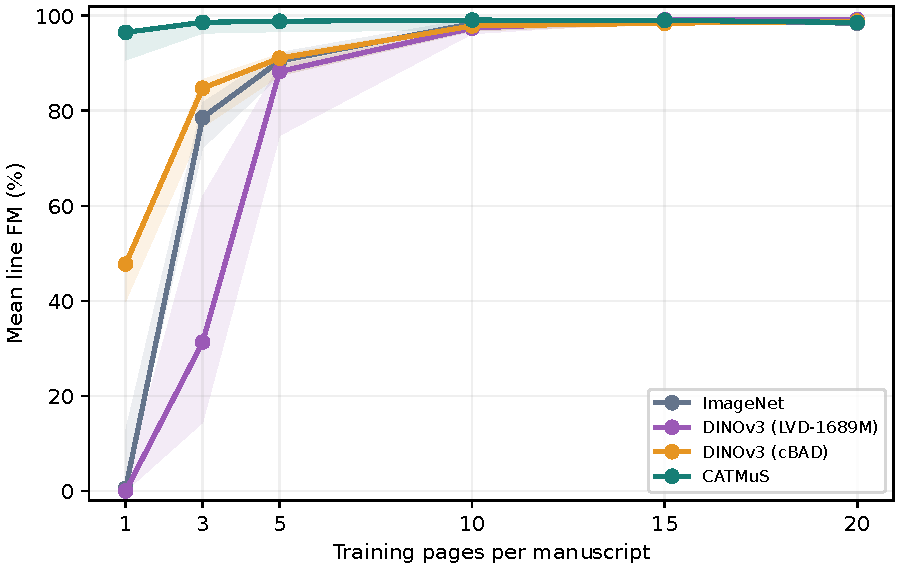
\includegraphics[width=0.75\linewidth]{graphics/rq2_pretraining_shots.pdf}
    \caption{Mask R-CNN (ConvNeXt-Tiny) on DIVA-HisDB: mean line \gls{fm} by number of training pages and initialization. Lines: random selection; shading: range over the six selection strategies.}
    \label{fig:rq2-pretraining-shots}
\end{figure}

\FloatBarrier

\section{Cross-Collection Transfer}
\label{sec:results-rq3}

In all three transfer settings, the center-line model transfers to new collections better than Mask R-CNN. Since the center-line decoding rules were selected on training and validation pages of the seven collections, zero-shot here means that the network weights are not fine-tuned on the target collection.

\FloatBarrier
\subsection{Zero-Shot Transfer}
\label{sec:results-rq3-zeroshot}

As shown in Table~\ref{tab:rq3-zeroshot}, the center-line model transfers well without fine-tuning. It reaches 91.67\%, compared with 44.26\% for Mask R-CNN, a difference of 47.4 percentage points. Mask R-CNN fails on GRPOLY-DB with 0.06\% and reaches only 20.64\% and 29.79\% on ONB Cod.\ Syr.\ 1 and NorHand v3. The center-line model stays above 83\% on every collection.

\begin{table}[htbp]
    \centering
    \caption{Zero-shot results of the CATMuS-pretrained models on the RQ3 collections.}
    \label{tab:rq3-zeroshot}\label{tab:rq3-zeroshot-center-line}
    \scriptsize
    \setlength{\tabcolsep}{2pt}
    \begin{tabular*}{\textwidth}{@{\extracolsep{\fill}}lrcccccccccc@{}}
        \toprule
        & & \multicolumn{5}{c}{Mask R-CNN} & \multicolumn{5}{c}{Center-line model} \\
        \cmidrule(lr){3-7}\cmidrule(l){8-12}
        Collection & Pages & Pixel IU & Line IU & DR & RA & FM & Pixel IU & Line IU & DR & RA & FM \\
        \midrule
        Pinkas & 6 & 82.04 & 63.77 & 73.86 & 81.79 & 77.54 & 90.14 & 72.49 & 81.03 & 87.23 & 83.97 \\
        ONB Cod.\ Syr.\ 1 & 123 & 52.28 & 12.37 & 20.63 & 21.41 & 20.64 & 98.52 & 89.19 & 91.02 & 97.86 & 94.12 \\
        RASAM & 462 & 74.84 & 54.33 & 69.19 & 62.29 & 64.68 & 92.57 & 87.92 & 92.18 & 94.42 & 92.94 \\
        RASM2018/2019 & 105 & 66.38 & 41.84 & 54.65 & 58.97 & 54.58 & 93.10 & 87.89 & 88.78 & 97.85 & 92.11 \\
        Phil.\ gr.\ 130 & 13 & 68.97 & 47.49 & 57.26 & 70.58 & 62.55 & 85.00 & 78.46 & 84.04 & 91.47 & 87.10 \\
        GRPOLY-DB & 38 & 19.77 & 0.03 & 0.16 & 0.04 & 0.06 & 99.47 & 96.44 & 100.00 & 96.44 & 98.15 \\
        NorHand v3 & 81 & 48.06 & 21.09 & 36.52 & 26.22 & 29.79 & 92.42 & 88.26 & 92.38 & 94.48 & 93.26 \\
        \midrule
        Mean & & 58.91 & 34.42 & 44.61 & 45.90 & 44.26 & 93.03 & 85.81 & 89.92 & 94.25 & 91.67 \\
        \bottomrule
    \end{tabular*}
\end{table}

\FloatBarrier
\subsection{Single-Collection Transfer}
\label{sec:results-rq3-protocol-a}

Fine-tuning on three pages of one collection improves Mask R-CNN in-domain, but its result drops on the other collections (Table~\ref{tab:rq3-matrix-ab-fm}). It reaches 88.61\% in-domain and 70.56\% on the other collections. Additionally, its result on GRPOLY-DB depends on the source collection.

\begin{table}[H]
    \centering
    \caption{Single-collection transfer matrix of Mask R-CNN (\gls{fm}).}
    \label{tab:rq3-matrix-ab-fm}
    \footnotesize
    \setlength{\tabcolsep}{3pt}
    \begin{tabular}{@{}l*{7}{r}rr@{}}
        \toprule
        & \multicolumn{7}{c}{Test collection} & \multicolumn{2}{c}{Mean} \\
        \cmidrule(lr){2-8}\cmidrule(l){9-10}
        Train & Pinkas & ONB & RASAM & RASM & Phil. & GRPOLY & NorHand & All & Transfer \\
        \midrule
        Pinkas & \cellcolor{gray!20}81.54 & 84.42 & 83.78 & 82.05 & 58.08 & 1.10 & 61.49 & 64.64 & 61.82 \\
        ONB & 84.76 & \cellcolor{gray!20}96.07 & 92.99 & 89.28 & 53.97 & 63.73 & 79.99 & 80.11 & 77.45 \\
        RASAM & 82.91 & 94.62 & \cellcolor{gray!20}94.01 & 91.31 & 50.11 & 92.32 & 77.26 & 83.22 & 81.42 \\
        RASM & 79.94 & 94.09 & 94.01 & \cellcolor{gray!20}90.55 & 38.32 & 18.77 & 69.26 & 69.28 & 65.73 \\
        Phil. & 83.05 & 78.07 & 81.12 & 76.35 & \cellcolor{gray!20}71.97 & 1.08 & 59.64 & 64.47 & 63.22 \\
        GRPOLY & 54.70 & 85.75 & 72.39 & 76.98 & 19.93 & \cellcolor{gray!20}99.30 & 58.25 & 66.76 & 61.33 \\
        NorHand & 77.14 & 93.48 & 90.11 & 85.95 & 52.51 & 98.25 & \cellcolor{gray!20}86.84 & 83.47 & 82.91 \\
        \midrule
        Transfer into & 77.08 & 88.41 & 85.73 & 83.65 & 45.49 & 45.88 & 67.65 & & \\
        \bottomrule
    \end{tabular}
\end{table}

The center-line model keeps most of its in-domain quality on the other collections (Table~\ref{tab:rq3-matrix-center-line-fm}). It reaches 93.97\% in-domain and 91.36\% transfer. Per target collection, it is 20.8 percentage points better than Mask R-CNN. Only one source--target pair, Pinkas\(\rightarrow\)Phil.\ gr.\ 130, falls below 82\%.

\begin{table}[htbp]
    \centering
    \caption{Single-collection transfer matrix of the center-line model (\gls{fm}).}
    \label{tab:rq3-matrix-center-line-fm}
    \footnotesize
    \setlength{\tabcolsep}{3pt}
    \begin{tabular}{@{}l*{7}{r}rr@{}}
        \toprule
        & \multicolumn{7}{c}{Test collection} & \multicolumn{2}{c}{Mean} \\
        \cmidrule(lr){2-8}\cmidrule(l){9-10}
        Train & Pinkas & ONB & RASAM & RASM & Phil. & GRPOLY & NorHand & All & Transfer \\
        \midrule
        Pinkas & \cellcolor{gray!20}85.04 & 92.92 & 92.74 & 90.79 & 69.86 & 96.82 & 83.49 & 87.38 & 87.77 \\
        ONB & 84.41 & \cellcolor{gray!20}95.34 & 93.81 & 92.00 & 91.17 & 97.69 & 93.01 & 92.49 & 92.02 \\
        RASAM & 86.48 & 94.79 & \cellcolor{gray!20}93.99 & 91.66 & 93.26 & 97.59 & 92.16 & 92.85 & 92.66 \\
        RASM & 83.83 & 95.24 & 93.93 & \cellcolor{gray!20}92.47 & 88.08 & 99.46 & 90.15 & 91.88 & 91.78 \\
        Phil. & 82.98 & 93.66 & 92.65 & 91.36 & \cellcolor{gray!20}97.37 & 97.59 & 91.31 & 92.42 & 91.59 \\
        GRPOLY & 83.74 & 95.91 & 93.35 & 92.46 & 91.27 & \cellcolor{gray!20}99.76 & 93.82 & 92.90 & 91.76 \\
        NorHand & 83.36 & 94.83 & 93.24 & 92.17 & 90.04 & 98.27 & \cellcolor{gray!20}93.80 & 92.24 & 91.98 \\
        \midrule
        Transfer into & 84.13 & 94.56 & 93.29 & 91.74 & 87.28 & 97.90 & 90.65 & & \\
        \bottomrule
    \end{tabular}
\end{table}

As shown in Table~\ref{tab:rq3-center-line-components}, \gls{wiseft} improves the transfer of the center-line model. Every interpolation transfers better than the fine-tuned model, and the mean transfer rises from 83.88\% at \(\alpha=1\) to 91.98\% at \(\alpha=0.25\). However, for Mask R-CNN, the best interpolation reaches 71.43\% at \(\alpha=0.75\), which is 0.87 percentage points above the fine-tuned model.

\begin{table}[htbp]
    \centering
    \caption{Effect of \gls{wiseft} on single-collection transfer (test pages, \gls{fm}). \(\alpha=0\): pretrained model; \(\alpha=1\): fine-tuned model.}
    \label{tab:rq3-center-line-components}\label{tab:rq3-wiseft}
    \footnotesize
    \begin{tabular}{@{}lcccc@{}}
        \toprule
        & \multicolumn{2}{c}{Center-line model} & \multicolumn{2}{c}{Mask R-CNN} \\
        \cmidrule(lr){2-3}\cmidrule(l){4-5}
        \(\alpha\) & Mean transfer & Lowest transfer & Mean transfer & Lowest transfer \\
        \midrule
        0.00 & 91.67 & \textbf{84.42} & 44.26 & 3.00 \\
        0.25 & \textbf{91.98} & 83.27 & 62.45 & 8.08 \\
        0.50 & 91.36 & 82.09 & 68.91 & 16.78 \\
        0.75 & 89.06 & 80.28 & \textbf{71.43} & \textbf{29.03} \\
        1.00 & 83.88 & 69.64 & 70.56 & 28.21 \\
        \bottomrule
    \end{tabular}
\end{table}

\FloatBarrier
\subsection{Leave-One-Collection-Out Transfer}
\label{sec:results-rq3-loco}

More annotated source pages improve the transfer of Mask R-CNN (Table~\ref{tab:rq3-locok}). From \gls{loco}-1 to \gls{loco}-3, its mean \gls{fm} on the held-out collections rises from 79.23\% to 85.44\%, and on Phil.\ gr.\ 130 from 25.77\% to 54.12\%. However, dense collections such as Phil.\ gr.\ 130 remain difficult. Since the six source collections stay the same, this comparison varies the number of annotated pages but not the diversity of the sources. The best source collection is chosen on the test results, so this value overestimates the result of a source chosen in advance.

\begin{table}[htbp]
    \centering
    \caption{\Gls{loco} results of Mask R-CNN on the held-out collections, with single-collection references (\gls{fm}).}
    \label{tab:rq3-locok}\label{tab:rq3-locok-maskrcnn}
    \footnotesize
    \setlength{\tabcolsep}{3pt}
    \begin{tabular}{@{}l*{7}{r}r@{}}
        \toprule
        & \multicolumn{7}{c}{Held-out collection} & Mean \\
        \cmidrule(lr){2-8}
        Training setting & Pinkas & ONB & RASAM & RASM & Phil. & GRPOLY & NorHand & All \\
        \midrule
        In-domain (A) & \cellcolor{gray!20}81.54 & \cellcolor{gray!20}96.07 & \cellcolor{gray!20}94.01 & \cellcolor{gray!20}90.55 & \cellcolor{gray!20}71.97 & \cellcolor{gray!20}99.30 & \cellcolor{gray!20}86.84 & 88.61 \\
        Best source (A) & 84.76 & 94.62 & 94.01 & 91.31 & 58.08 & 98.25 & 79.99 & 85.86 \\
        \midrule
        \gls{loco}-1 & 82.05 & 93.64 & 92.33 & 87.97 & 25.77 & 94.35 & 78.46 & 79.23 \\
        \gls{loco}-2 & 80.63 & 93.28 & 92.20 & 88.07 & 40.28 & 98.49 & 86.37 & 82.76 \\
        \gls{loco}-3 & 80.32 & 93.97 & 92.47 & 90.77 & 54.12 & 99.33 & 87.12 & 85.44 \\
        \bottomrule
    \end{tabular}
\end{table}

The number of source pages has little effect on the center-line model (Table~\ref{tab:rq3-loco3-center-line}). It reaches 91.82\% with \gls{loco}-1 and 92.64\% with \gls{loco}-3. Additionally, its result stays between 91.36\% and 92.64\% in all transfer settings. The remaining difference to Mask R-CNN comes mainly from Phil.\ gr.\ 130, with 92.07\% compared with 54.12\%. On GRPOLY-DB, ONB Cod.\ Syr.\ 1, and RASAM, both models are within one percentage point. Section~\ref{sec:disc-failures} analyzes the errors behind these results.

\begin{table}[htbp]
    \centering
    \caption{\Gls{loco} results of the center-line model on the held-out collections, with single-collection references (\gls{fm}).}
    \label{tab:rq3-loco3-center-line}\label{tab:rq3-locok-center-line}
    \footnotesize
    \setlength{\tabcolsep}{3pt}
    \begin{tabular}{@{}l*{7}{r}r@{}}
        \toprule
        & \multicolumn{7}{c}{Held-out collection} & Mean \\
        \cmidrule(lr){2-8}
        Training setting & Pinkas & ONB & RASAM & RASM & Phil. & GRPOLY & NorHand & All \\
        \midrule
        In-domain (A) & \cellcolor{gray!20}85.04 & \cellcolor{gray!20}95.34 & \cellcolor{gray!20}93.99 & \cellcolor{gray!20}92.47 & \cellcolor{gray!20}97.37 & \cellcolor{gray!20}99.76 & \cellcolor{gray!20}93.80 & 93.97 \\
        \midrule
        \gls{loco}-1 & 83.13 & 94.36 & 92.90 & 91.96 & 94.23 & 96.66 & 89.47 & 91.82 \\
        \gls{loco}-2 & 83.97 & 94.61 & 92.78 & 91.83 & 93.56 & 98.79 & 91.06 & 92.37 \\
        \gls{loco}-3 & 85.81 & 94.24 & 93.34 & 92.29 & 92.07 & 98.96 & 91.74 & 92.64 \\
        \bottomrule
    \end{tabular}
\end{table}

\endgroup
